%Especificacion
\documentclass[12pt]{article}

%Paquetes
\usepackage[left=2cm,right=2cm,top=3cm,bottom=3cm,letterpaper]{geometry}
\usepackage{lmodern}
\usepackage[T1]{fontenc}
\usepackage[utf8]{inputenc}
\usepackage[spanish,activeacute, es-nodecimaldot]{babel}
\usepackage{mathtools}
\usepackage{amssymb}
\usepackage{enumerate}
\usepackage{graphicx}
\usepackage{titlesec}
\usepackage{enumitem}
\usepackage{alltt}
\usepackage{hyperref}
\usepackage{algorithm}
\usepackage{algorithmic}
\usepackage[export]{adjustbox}

%Preambulo
\title{Seminario de Heurísticas de Optimización Combinatoria}
\author{Heurística de opitmización Binary Fish School Search \\ aplicada al problema Subset Sum}
\date{Andrea Itzel González Vargas \\ $\ $ \\ Facultad de Ciencias \\ UNAM}

\setlength\parindent{0pt}

\begin{document}
\maketitle
\tableofcontents
\newpage

\section{Introducción}
Para este proyecto se eligió la heurística llamada \hyperref[sec:bfss]{Binary Fish School Search} (BFSS) para resolver el problema NP-completo \hyperref[sec:ss]{Subset Sum}. BFSS es una modificación de la heurística Fish School Search (FSS) que utiliza vectores binarios para simular una posible solución a una instancia, a diferencia de FSS donde se utiliza un número flotante. Por la naturaleza del problema Subset Sum se decidió optar por usar BFSS sobre FSS. \\

Se utlizó el lenguaje de programación Go en su versión 1.8 para la implementación del proyecto, se creó además una interfaz gráfica que permite visualizar el estado del programa mientras se ejecuta. El repositorio del proyecto se encuentra en \url{https://github.com/andreagonz/peces}. 

\section{Compilación y ejecución}

\subsection{Compilación}
Para poder compilar el programa se requiere tener instalada al menos la versión 1.7 de Go. \footnote{Se recomienda tener la versión 1.8 de Go: \url{https://golang.org/doc/go1.8}} \\
Se necesita además instalar paquetes adicionales de Go con los comandos:
\begin{verbatim}
    $ go get -u github.com/asticode/go-astilectron
    $ go get github.com/julienschmidt/httprouter
    $ go get -u github.com/jteeuwen/go-bindata/...
\end{verbatim}
Desde la carpeta \textsf{go/src/github.com/andreagonz/peces} se debe ejecutar el siguiente comando:
\begin{verbatim}
    $ go build
\end{verbatim}

\subsection{Ejecución}
Para ejecutar el programa se debe de correr el comando:
\begin{verbatim}
    $ ./peces <archivo.ss> <params.txt> [-gui]
\end{verbatim}
donde \texttt{<archivo.ss>} es el archivo donde se especifica la instancia del problema a resolver. El formato de éste es el siguiente:  \\

\texttt{int: Suma a buscar} \\
$\texttt{int:x}_{\texttt{1}},\ \texttt{int:x}_{\texttt{2}},\ ...,\ \texttt{int:x}_{\texttt{n}}$ \\

Donde \texttt{int: Suma a buscar} es un número entero que representa la suma del subconjunto que se quiere encontrar (más detalles en la \hyperref[sec:ss]{siguiente sección}), y cada $\texttt{int:x}_{\texttt{i}}$ es un número entero, que representa un elemento del conjunto de números entrada, cada número va separado por una coma.

\newpage

Ejemplo:
\begin{verbatim}
13
0, 3, -1, 10
\end{verbatim}
En este ejemplo se busca el subconjunto de números en $\{0, 3, -1, 10\}$ que sumen $13$, o sea $\{10, 3\}$. \\

En el archivo \texttt{<params.txt>} deben venir especificados los parámetros a ser utilizados para la heurística. Debe de tener el siguiente formato: \\

%%%%%%%%NOMBRES DE PARAMETROS
\texttt{int: Semilla} \\
\texttt{int: Número de iteraciones} \\
\texttt{int: Tamaño del cardumen} \\
\texttt{double: $\texttt{step}_{\texttt{ind}}$} \\
\texttt{double: $\texttt{prob}_{\texttt{ind}}$} \\
\texttt{double: $\texttt{thres}_{\texttt{c}}$} \\
\texttt{double: $\texttt{thres}_{\texttt{v}}$} \\

Ejemplo:
\begin{verbatim}
3
100
49
0.9
0.001
0.9
0.9
\end{verbatim}

En la \hyperref[sec:bfss]{sección 4} se explica qué significan estos parámetros. \\

Finalmente, \texttt{[-gui]} es un parámetro opcional que de ser utilizado mostrará una interfaz gráfica para ejecutar el programa visualmente.\footnote{Cuando se usa por primera vez la opción \texttt{-gui} puede que el programa tarde en ejecutarse.} En la carpeta \texttt{archivos/} se encuentran algunas instancias de problemas y parámetros que pueden ser utilizados para la ejecución del programa. Ejemplo:
\begin{verbatim}
    $ ./peces archivos/5.ss archivos/params1.txt -gui
\end{verbatim}

Una vez ejecutado el programa se crea el archivo \texttt{subconjunto.res} donde se muestra el mejor subconjunto resultante de la búsqueda.

\newpage

\section{Problema Subset Sum} \label{sec:ss}
El problema Subset Sum consiste en que se tiene un conjunto de números enteros y se quiere encontrar un subconjunto no vacío tal que la suma de todos los elementos de éste sean un número $x$ dado, si es que no existe tal subconjunto, se quiere encontrar el subconjunto que de la suma que se aproxime lo más posible a $x$. Subset Sum se puede ver como un caso especial del problema Knapsack. \\

La dificultad de este problema radica en que no se conoce un algoritmo que en todos los casos nos de una solución al problema de manera eficiente, por lo que se hace uso de heurísticas para hacer aproximaciones.

\section{Heurística Binary Fish School Search } \label{sec:bfss} 
Esta heurística está basada en el movimiento de los peces en cardumenes que van en busca de comida. Cada pez representa una solución candidata al problema y tiene asociado un $peso$ y un $fitness$. Cuando un pez encuentra un lugar con alimento abundante (una buena solución que determinará al fitness de este pez), su peso aumenta en proporción a la cantidad de alimento (el fitness) utilizando un \textbf{operador de alimentación}. Hay tres tipos de movimientos en la heurística, cada uno representa un operador:
\begin{itemize}
\item \textbf{Movimiento individual:} Cada pez se mueve aleatoriamente.
\item \textbf{Movimiento colectivo instintivo:} El cardumen sigue a los peces con más fitness.
\item \textbf{Movimiento colectivo volitivo:} El cardumen sigue a los peces con más peso (aquellos que han ido encontrado mejores soluciones).
\end{itemize}

El algoritmo del BFSS (y en general del FSS) es el siguiente: 

\begin{algorithm}                     
\caption{Binary Fish School Search}         
\label{alg1}                           
\begin{algorithmic}
	\STATE Inicializar parámetros y cardumen
  	\STATE Inicializar posiciones de peces aleatoriamente
  	\WHILE {\NOT Condición de paro}
        	\STATE Calcular fitness de cada pez
        	\STATE Correr operador de movimiento individual
                \STATE Calcular fitness de cada pez
                \STATE Correr operador de alimentación
                \STATE Correr operador de movimiento colectivo instintivo
                \STATE Correr operador de movimiento colectivo volitivo
	\ENDWHILE
\end{algorithmic}
\end{algorithm}

A continuación se explicará cómo es que se implementó cada operador.

\newpage

\subsection{Implementación}
La implementación se hizo basándose en el artículo \cite{articulo} con algunos cambios.

\subsubsection{Codificación}
Un cardumen $Car$ es un arreglo de peces, cada pez $p_i \in Car$ tiene asignado un vector binario $v_i = [v_{i1}, v_{i2},...,v_{in}]$ donde cada $v_{ij} \in \{0, 1\}$. Este vector representa la posición del $p_i$ y es una posible solución, tal que si se tiene una instancia del problema Subset Sum con un vector $x = [ x_1, x_2,...,x_n]$ que representa al conjunto $C$ de la instancia, entonces $v_i$ representa un subconjunto $S_i$ de $C$, donde si $v_{ij} = 0$ entonces $x_j \notin S_i$ y si $v_{ij} = 1$ entonces $x_j \in S_i$.

\subsubsection{Función de fitness}
Para cada pez $p_i \in Car$, dado $S_i$ (que como se había indicado previamente es el subconjunto de $C$ que representa $p_i$), sea $sum_i = \sum\limits_{x \in S_i}x$ y $sum$ la suma que se quiere aproximar lo más posible, el fitness $f_i$ de $p_i$ se definió como $f_i = 1 - \frac{|sum_i - sum|}{max_{\Delta}}$ donde $max_{\Delta} = max\{\Delta_{max}, \Delta_{min}\}$ y a su vez $\Delta_{max}$ es la diferencia entre la mayor suma posible (de elementos del conjunto $C$) y $sum$, análogamente $\Delta_{min}$ es la diferencia entre la menor suma posible y $sum$.

\subsubsection{Condición de paro}
La condición de paro consiste simplemente en que el programa se detenga cuando se llegue a cierto número de iteraciones o se encuentra algún subconjunto con la suma buscada.

\subsubsection{Inicialización de posiciones}
La posición inicial de cada pez $p_i$ se inicializa de manera aleatoria, dado $v_i$ de $p_i$, cada entrada $v_{ij}$ se decide con la siguiente función:
\begin{equation*}
  v_{ij} =
  \begin{cases*}
      1 & si $r > 0.5$ \\
      0 & en otro caso 
    \end{cases*}
\end{equation*}
donde $r$ es un número aleatorio uniformemente distribuido entre 0 y 1.

\subsubsection{Operador de alimentación}
Sea $W_i(t)$ el peso de $p_i$ en la iteración $t$, entonces $W(t + 1)$ se define como:
\begin{equation*}
  W_i(t + 1) = W_i(t) + \frac{\Delta f_i}{max(|\Delta f_j|)}
\end{equation*}
Donde $\Delta f_i$ es la diferencia de fitness entre la última posición y la actual de $p_i$, y $max(|\Delta f_j|)$ representa la $\Delta f_j$ cuyo valor absoluto es el mayor entre el de todos los peces.

\subsubsection{Operador de movimiento individual}
El vector $v_i$ de $p_i$ se modifica de la siguiente manera. Para cada $v_{ij}$:
\begin{equation*}
  v_{ij} =
  \begin{cases*}
    \overline{v_{ij}} & si $r < step_{ind}(t)$ \\
    v_{ij} & en otro caso 
  \end{cases*}
\end{equation*}
En el artículo el pez cambia de posición sólo si su fitness mejora, sin embargo según la experimentación hecha esto limita la capacidad de exploración, por lo que se introduce el parámetro $prob_{ind}$, tal que dado otro número $r'$ unformememnte distribuido ente 0 y 1, si $r' < prob_{ind}$ al pez se le permite cambiar de posición sin importar si mejora su fitness. \\

Definimos $step_{ind} = step_{ind}(0)$, donde $step_{ind}$ es un parámetro de la heurística. $step_{ind}(t)$ es un valor que decrece mientras $t$ aumenta, de acuerdo a la función:
\begin{equation*}
  step_{ind}(t + 1) = step_{ind}(t) - \frac{step_{ind}}{It_{max}}
\end{equation*}
donde $It_{max}$ es el número máximo de iteraciones a correr.

\subsubsection{Operador de movimiento colectivo instintivo}
Se crea el vector $I(t) = [u_1, u_2,...,u_n]$ que afectará el movimiento de todos los peces.
\begin{equation*}
  I(t) = \frac{\sum_{i=1}^nv_i\Delta f_i}{\sum_{i=1}^n\Delta f_i}
\end{equation*}
Esto significa que para crear $I(t)$, cada vector $v_i$ de los peces es multiplicado por $\Delta f_i$, se suman todos los vectores resultantes y el resultado se divide entrada por entrada entre $\sum_{i=1}^n\Delta f_i$. El resultado es que $I(t)$ es un vector de numeros flotantes entre 0 y 1, se convierte entonces a $I(t)$ en un  vector binario usando el parámetro $thres_c$, que es un número entre 0 y 1.
\begin{equation*}
  u_i =
  \begin{cases*}
    0 & si $u_i < thres_c \times max\{u_j\}$ \\
    1 & en otro caso 
  \end{cases*}
\end{equation*}
para cada $u_i$ de $I(t)$, donde $max\{u_j\}$ es la $u_j$ mayor entre todos los elementos de $I(t)$. \\

Por último, el vector $v_i$ de cada pez $p_i$ es modificado de la siguiente manera. Se escoge alguna entrada $v_{ij}$ de $v_i$ aleatoriamente tal que $v_{ij} \neq u_j$ y se modifica por su complemento, tal que $v_{ij} = u_j$.

\subsubsection{Operador de movimiento colectivo volitivo}
Similarmente al movimiento anterior, se crea un vector $B(t) = [u_1, u_2,...,u_n]$ que modificará la posición de los peces.
\begin{equation*}
  B(t) = \frac{\sum_{i=1}^nv_i W_i(t)}{\sum_{i=1}^n W_i(t)}
\end{equation*}
Se usa el parámetro $thres_v$ para volver a $B(t)$ un vector binario, para cada entrada $u_i$:
\begin{equation*}
  u_i =
  \begin{cases*}
    0 & si $u_i < thres_v(t) \times max\{u_j\}$ \\
    1 & en otro caso 
  \end{cases*}
\end{equation*}
Si el peso en conjunto de todos los peces en la iteración anterior comparado con la iteración actual mejoró, entonces $B(t)$ se queda tal y como está, de lo contrario se modifica de manera que $B(t) = [\overline{u_1}, \overline{u_2},...,\overline{u_n}]$. \\

Para finalizar, para cada $v_i$ se escoge una entrada $v_{ij}$ tal que $v_{ij} \neq u_j$ y se cambia por su complemento. \\

$thres_v(t)$ al igual que $step_{ind}(t)$ disminuye mientras $t$ aumenta. Definimos $thres_v = thres_v(0)$. $thres_v$ decrece de acuerdo a la función:
\begin{equation*}
  thres_v(t + 1) = thres_v(t) - \frac{thres_v}{It_{max}}
\end{equation*}

\section{Ejemplo de la ejecución de una instancia}
Al ejecutar el comando
\begin{verbatim}
    $ ./peces archivos/5.ss archivos/params1.txt
\end{verbatim}

se imprime en terminal los siguientes resultados
\begin{verbatim}
Tamaño de conjunto inicial: 10000
Suma a buscar: -11207948

Resultado 
Mejor suma encontrada: -11207946
Tamaño de conjunto: 4996
Fitness: 0.9999999998025653
\end{verbatim}

y en el archivo \texttt{subconjunto.res} se guarda el mejor subconjunto encontrado. \\

Al ejecutar

\begin{verbatim}
    $ ./peces archivos/4.ss archivos/params1.txt -gui
\end{verbatim}

se abre la interfaz gráfica y se muestra lo siguiente: \\
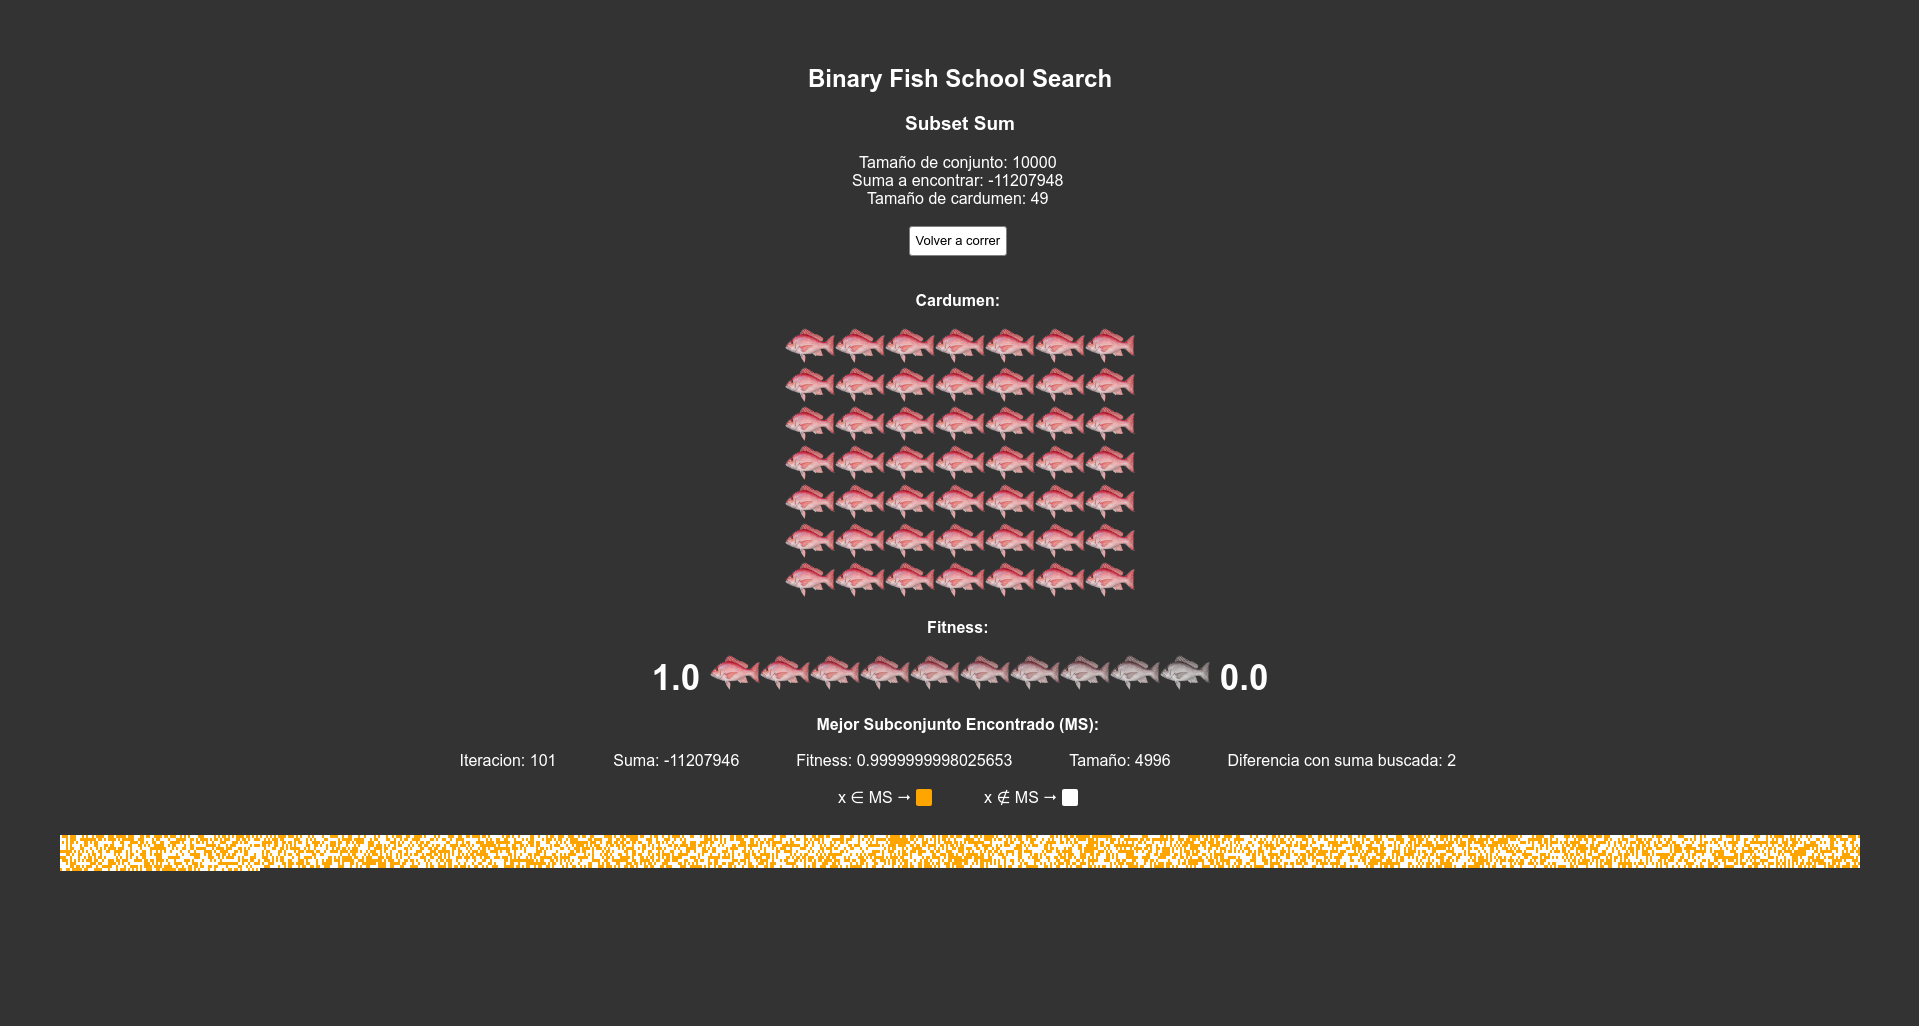
\includegraphics[scale=0.262]{media/gui} \\

donde los peces representan el cardumen y el color de cada pez su fitness, mientras más grises sean los peces peor será su fitness. La franja color naranja y blanco representa el conjunto de la instancia del problema, los cuadros de color naranja representan los elementos que están en el mejor subconjunto encontrado y los de color blanco los que no. 

\section{Experimentación}

Se usó el programa \texttt{otros/generador.py} para crear instancias del problema. Para utilizarlo se debe ejecutar de la siguiente manera.
\begin{verbatim}
    $ python3 generador.py <Num. de elementos> [Semilla] [Cota minima] [Cota maxima]
\end{verbatim}

donde \texttt{<Num. de elementos>} es el número de elementos que se quiere meter en el conjunto. \texttt{[Semilla] [Cota minima] y [Cota maxima]} son parámetros opcionales, respectivamente son la semilla que se utilizará para el generador pseudoaleatorio, la cota mínima de los números a meter en el conjunto y la cota máxima. Por defecto la semilla es 0, la cota mínima es -10000 y la máxima es 10000. \\

Para hacer los experimentos se utilizó una computadora con las características
\begin{verbatim}
Memoria RAM: 7.7GiB 
Procesador: Intel® Core™ i7-3630QM CPU @ 2.40GHz x 8 
\end{verbatim}

Los archivos utilizados se encuentran en la carpeta \texttt{archivos/}. \\
Primero se corrió el programa con conjuntos ``densos'', es decir, conjuntos cuyos elementos cubren un rango de números sin dejar muchos espacios entre sí. Se probó con conjuntos de 967, 19864, 40000 y 100000 (\texttt{1.ss}, \texttt{2.ss}, \texttt{3.ss} y \texttt{4.ss} respectivamente) elementos, cada conjunto se corrió 100 veces con distintas semillas (de 0 a 99), con los parámetros \texttt{params1.txt}, es decir: \\

$Número\ de\ iteraciones$: 100 \\
$Tamaño\ de\ cardumen$: 49 \\
$step_{ind}$: 0.9 \\
$prob_{ind}$: 0.001 \\
$thres_c$: 0.9 \\
$thres_v$: 0.9 \\

Los resultados fueron que en todos los casos se encontró el subconjunto con la suma deseada. El tiempo que tomó ejecutar las 100 semillas para cada conjunto fue:

\begin{itemize}
\item 967 elementos : 3.184 seg
\item 19864 elementos : 34.248 seg
\item 40000 elementos : 1 min 13.033 seg
\item 100000 elementos : 2 min 18.694 seg
\end{itemize}

Como este tipo de conjuntos no son muy interesantes, se probó el programa con conjuntos menos ``densos'', como el del archivo \texttt{5.ss}, que tiene 10000 elementos. Primero se probó con los parámetros de \texttt{params1.txt}, al igual que en el caso anterior se corrieron 100 semillas. El tiempo de ejecución fue mayor que en los casos anteriores (tardó 12 min 45.458 seg en correr las 100 semillas) ya que en algunos casos no se alcanzó la suma, por lo que se tuvo que realizar todas las iteraciones. La siguiente gráfica muestra la distancia entre la suma que se quiere encontrar y la mejor suma encontrada con respecto a las semillas utilizadas en cada ejecución: \\

\begin{center}
  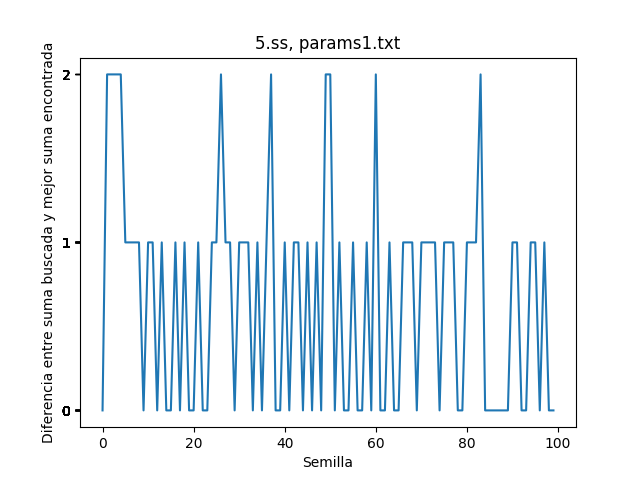
\includegraphics[scale=0.6]{media/5p1} \\
\end{center}

Recordemos que se le agregó el parámetro $prob_{ind}$ a la heruística original. Cuando éste se omite (se hace 0, usando \texttt{params2.txt}), entonces tenemos resultados muy diferentes a los anteriores, empezando por el tiempo de ejecución, que fue mayor (tardó 17 min 39.119 seg en correr 100 semillas):

\hspace*{-2cm}  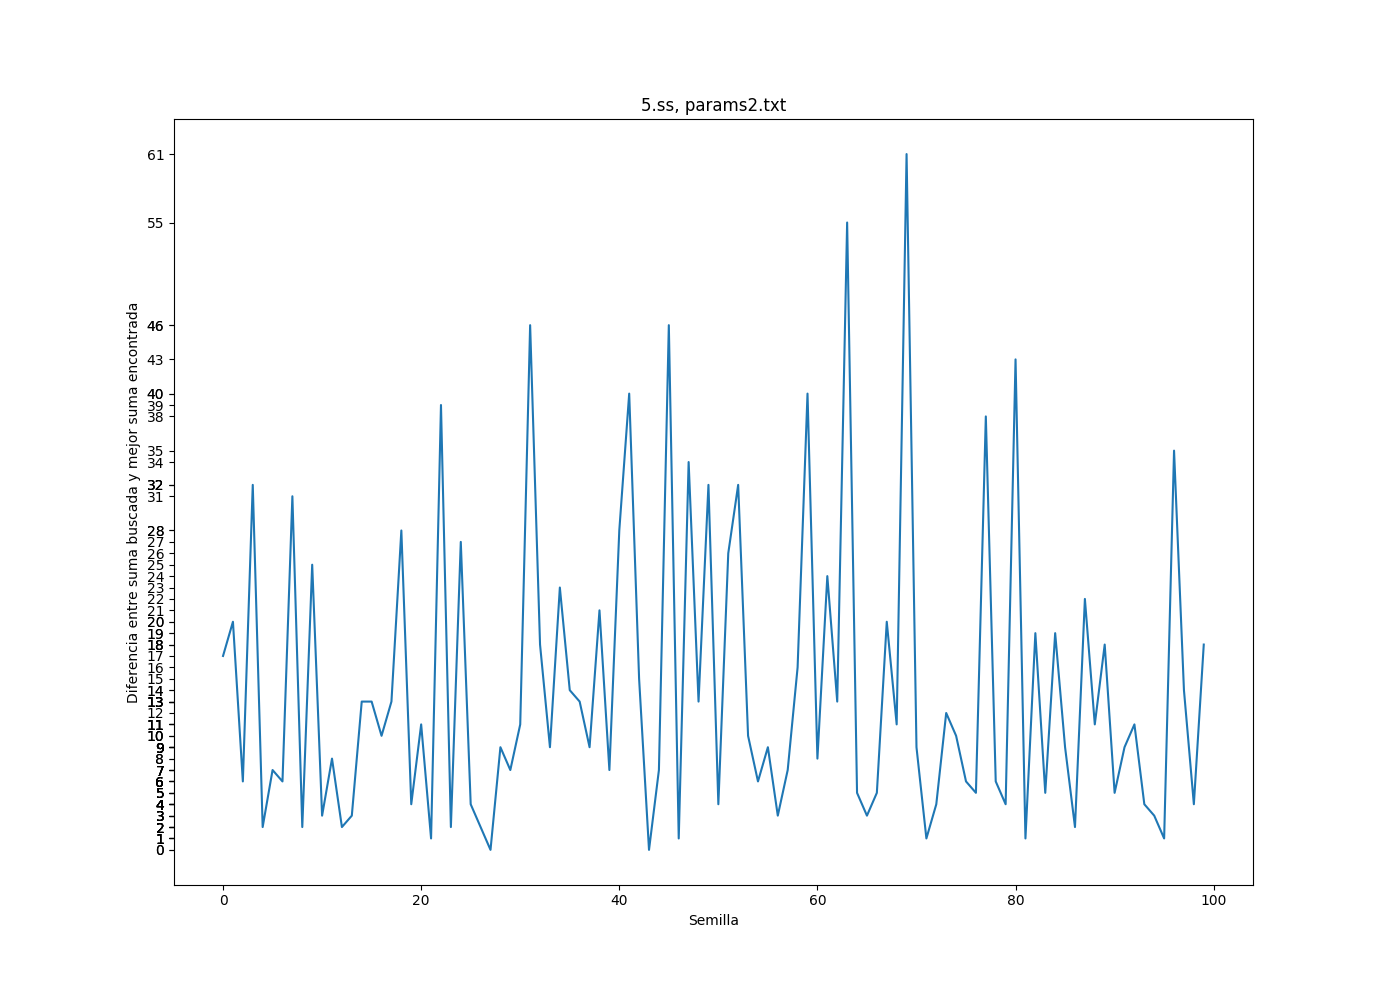
\includegraphics[scale=0.6]{media/5p2} \\

Vemos una variación mucho mayor entre la diferencia de sumas. \\

Por último se corrió un conjunto con 50000 elementos (\texttt{6.ss}) con 50 semillas distintas utlizando \texttt{params1.txt}, lo cual tomó 32 min 37.75 seg. Este conjunto consiste de números entre -10,000,000 y 10,000,000. Se generó la siguiente gráfica:

\begin{center}
  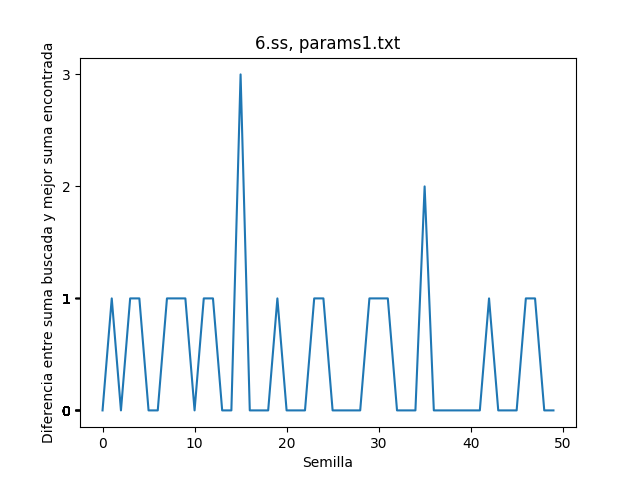
\includegraphics[scale=0.6]{media/6p1} \\
\end{center}

Todas estas imágenes se encuentran guardadas en la carpeta \texttt{documentos/media}.

\section{Análisis de resultados}
Los conjuntos que llamamos ``densos'' tuvieron resultados muy buenos, incluso con un conjunto tan grande como el de 100000 elementos se logró encontrar la suma buscada con todas las semillas y en muy poco tiempo. Con conjuntos menos ``densos'' se logró también tener resultados muy buenos al añadir el parámetro $prob_{ind}$, sin éste la diferencia entre la suma buscada y la mejor encontrada puede variar mucho más, ya que no se permite que se haga mucha exploración en el espacio de búsqueda.

\section{Conclusiones}
Si tuviera que resolver el problema Subset Sum en la vida real, definitivamente usaría la heurística BFSS, ya que se desempeñó muy bien incluso con conjuntos muy grandes y no tan ``densos''. Me sorpendió que se lograra obtener tan buenos resultados con tal sólo 49 peces en 100 iteraciones, ya que en mi experiencia con otras heurísticas, para obtener resultados decentes se necesita de al menos 1000 iteraciones y una población de mínimo 200 individuos o partículas, claro que todo depende del problema que se esté resolviendo, al parecer BFSS funciona muy bien para Subset Sum pero podría ser muy malo para otro tipo de problemas. \\

Sobre la implementación del proyecto, el programar la heurística no dio problemas mayores, y la función de costo fue fácil de crear ya que se sabe cuál es el resultado que se busca, a diferencia de otros problemas. \\

La parte de la implementación que se me complicó más fue la interfaz gráfica, ya que los proyectos de Go destinados a este fin no están completos o incluso abandonados, por la razón de que se destinan más recursos al desarrollo web. Por suerte encontré un proyecto para creación de interfaces gráficas en Go que es sencillo de usar y tiene las cosas básicas necesarias, que aunque parece que podría dificultarse su uso para proyectos más grandes, para un proyecto pequeño como este no causó tantos problemas, además de que la creación de la vista es muy fácil ya que se utiliza CSS, HTML y Javascript.

\begin{thebibliography}{99}

\bibitem{articulo}
  João André Gonçalves Sargo,
  \emph{Binary Fish School Search applied to Feature Selection},
  Master of Science Degree, Técnico Lisboa,
  Noviembre 2013. \\
  \url{https://fenix.tecnico.ulisboa.pt/downloadFile/395146003739/disserta%C3%A7%C3%A3o.pdf}
  \end{thebibliography}

  
\begin{figure}[b]
  
\includegraphics[scale=4, right]{media/gopherswim.jpg} \\
\end{figure}

\end{document}